\documentclass[11pt,a4paper]{article}

\usepackage[a4paper,margin=2.2cm]{geometry}
\usepackage[T1]{fontenc}
\usepackage[utf8]{inputenc}
\usepackage{lmodern}
\usepackage{microtype}
\usepackage{amsmath}
\usepackage{amssymb}
\usepackage{booktabs}
\usepackage{tabularx}
\usepackage{multirow}
\usepackage{graphicx}
\usepackage{subcaption}
\usepackage{xcolor}
\usepackage{float}
\usepackage{siunitx}
\usepackage{hyperref}
\usepackage[nameinlink,noabbrev]{cleveref}
\usepackage{listings}
\usepackage{enumitem}

\hypersetup{
  colorlinks=true,
  linkcolor=blue,
  citecolor=blue,
  urlcolor=blue,
  pdftitle={Optimization of a Hybrid Parallel D2Q9 Lattice Boltzmann Solver},
  pdfauthor={Your Name and Teammate Name}
}

\sisetup{
  detect-all,
  group-separator={,},
  group-minimum-digits=4
}

\title{Optimization of a Hybrid Parallel D2Q9 Lattice Boltzmann Solver for K\'arm\'an Vortex Street}
\author{Your Name \and Teammate Name}
\date{\today}

\begin{document}

\maketitle
\tableofcontents
\newpage

\section{Introduction}

This report presents the optimization of a hybrid MPI+OpenMP D2Q9 lattice Boltzmann solver for the simulation of a K\'arm\'an vortex street. The objective was to improve both performance and scalability while preserving the correctness of the physical simulation.

The optimization process followed a systematic workflow: identify a bottleneck using profiling tools, implement a targeted optimization, measure its impact, and validate numerical correctness. Both successful and unsuccessful attempts are reported, since negative results provided useful insights into the true performance constraints of the code.

The optimized source code is available at:
\begin{center}
\url{https://github.com/FANG-leo/TOP.git}
\end{center}

\section{Experimental Methodology}

\subsection{Benchmark Configuration}

Unless stated otherwise, benchmarks were performed using the reference problem described by the following configuration:
\begin{itemize}[leftmargin=1.5em]
  \item iterations: \texttt{20000}
  \item width: \texttt{800}
  \item height: \texttt{160}
  \item obstacle position: \texttt{(100.0, 80.0)}
  \item obstacle radius: \texttt{12.0}
  \item Reynolds number: \texttt{96}
  \item inflow maximum velocity: \texttt{0.16}
\end{itemize}

The main performance metric used throughout this report is the figure of merit reported by the application, expressed in MLUPS (million lattice updates per second). We also use elapsed time, speedup, parallel efficiency, hotspot sampling, and hardware-counter statistics.

For scalability analysis, we distinguish between strong scaling and weak scaling. Strong scaling refers to increasing the number of processing elements while keeping the global problem size fixed. Weak scaling refers to increasing both the problem size and the number of processing elements so that the amount of work per processing element remains approximately constant.

\subsection{Validation Strategy}

All optimized versions were checked against the reference behavior to ensure that performance improvements did not alter the numerical results. Validation was performed using the provided visualization and comparison tool, by comparing generated outputs against the baseline reference file.

\subsection{Data Sources}

Two sets of measurements were used:
\begin{itemize}[leftmargin=1.5em]
  \item the optimization logs and step-by-step performance observations collected during development;
  \item an extended benchmark matrix collected on a second machine and stored in the \texttt{perf-data} directory.
\end{itemize}

Because the two systems are not identical, absolute MLUPS values are only compared within the same machine. Across machines, only relative speedups and qualitative trends are compared.

\section{System Configuration}

\subsection{Hardware and Software Environment}

Table~\ref{tab:system-config} summarizes the system configuration used for the local benchmark campaign.

\begin{table}[H]
  \centering
  \caption{Benchmark platform configuration.}
  \label{tab:system-config}
  \begin{tabularx}{\textwidth}{@{}lX@{}}
    \toprule
    Component & Description \\
    \midrule
    CPU & AMD Ryzen 9 7940HX, 16 cores, 32 threads, up to \SI{5.31}{GHz} \\
    SIMD ISA & AVX2, AVX-512 class extensions available \\
    Cache hierarchy & L1d: \SI{512}{KiB}, L2: \SI{16}{MiB}, L3: \SI{64}{MiB} \\
    Memory & \SI{30}{GiB} RAM \\
    OS & Ubuntu 24.04, Linux kernel \texttt{6.17.0-22-generic} \\
    Compiler & GCC 13.3.0 \\
    CMake & 3.28.3 \\
    MPI & Open MPI 4.1.6 \\
    Parallel programming models & MPI 3.0+, OpenMP 4.0+ \\
    Build mode & \texttt{Release}, with \texttt{-march=native} \\
    \bottomrule
  \end{tabularx}
\end{table}

\section{Baseline Analysis}

\subsection{Initial Profiling}

Initial profiling showed that the solver runtime was dominated by two computational kernels:
\begin{itemize}[leftmargin=1.5em]
  \item \texttt{collision()}
  \item \texttt{propagation()}
\end{itemize}

These kernels remained the main hotspots throughout the project and therefore became the primary optimization targets. In addition, the MPI version exhibited inefficient halo exchanges and excessive synchronization.

\subsection{Representative Early Hotspots}

Table~\ref{tab:baseline-hotspots} shows a representative early hotspot decomposition. It illustrates the initial dominance of \texttt{collision()} and \texttt{propagation()}, which motivated the first rounds of single-core tuning.

\begin{table}[H]
  \centering
  \caption{Representative hotspot breakdown for an optimized MPI-oriented configuration.}
  \label{tab:baseline-hotspots}
  \begin{tabular}{@{}lr@{}}
\toprule
Symbol & Samples (\%) \\
\midrule
main & 73.34 \\
collision(Mesh*, Mesh const*) & 37.40 \\
propagation(Mesh*, Mesh const*) & 26.15 \\
lbm\_comm\_halo\_exchange(lbm\_comm\_t\_s*, Mesh*) & 6.38 \\
PMPI\_Sendrecv & 5.09 \\
mca\_pml\_ob1\_send & 4.63 \\
opal\_progress & 2.51 \\
\_\_memmove\_avx512\_unaligned\_erms & 2.66 \\
\bottomrule
\end{tabular}

\end{table}

\subsection{Baseline Performance Table}

Table~\ref{tab:baseline-results} summarizes the early and later single-run reference points used in the version-evolution analysis.

\begin{table}[H]
  \centering
  \caption{Reference version evolution from the initial baseline to the final single-run point.}
  \label{tab:baseline-results}
  \begin{tabularx}{\textwidth}{@{}llr@{}}
\toprule
Version & Main change & FOM (MLUPS) \\
\midrule
v1 &  & 19.01 \\
v2 &  & 39.41 \\
v3 & Collision optimization & 58.17 \\
v4 & Propagation optimization & 65.87 \\
v5 & Further single-core tuning & 101.02 \\
v6 & SoA refactor & 227.67 \\
v7 & -march=native build & 223.08 \\
v8 & High-performance serial baseline & 218.74 \\
v9 & OpenMP-heavy attempt & 221.23 \\
v10 & Aligned allocation and pointer walk & 213.41 \\
v11 & MPI communication repair & 224.95 \\
v12 & Post-MPI cleanup and scaling study & 221.78 \\
\bottomrule
\end{tabularx}

\end{table}

\section{Optimization Process}

\subsection{Version-by-Version Evolution}

Figure~\ref{fig:version-evolution} summarizes the global performance evolution from the early baseline to the final optimized implementation. This figure should be read as a version-by-version progression of the reference benchmark, showing how successive optimizations progressively increased solver throughput.

\begin{figure}[H]
  \centering
  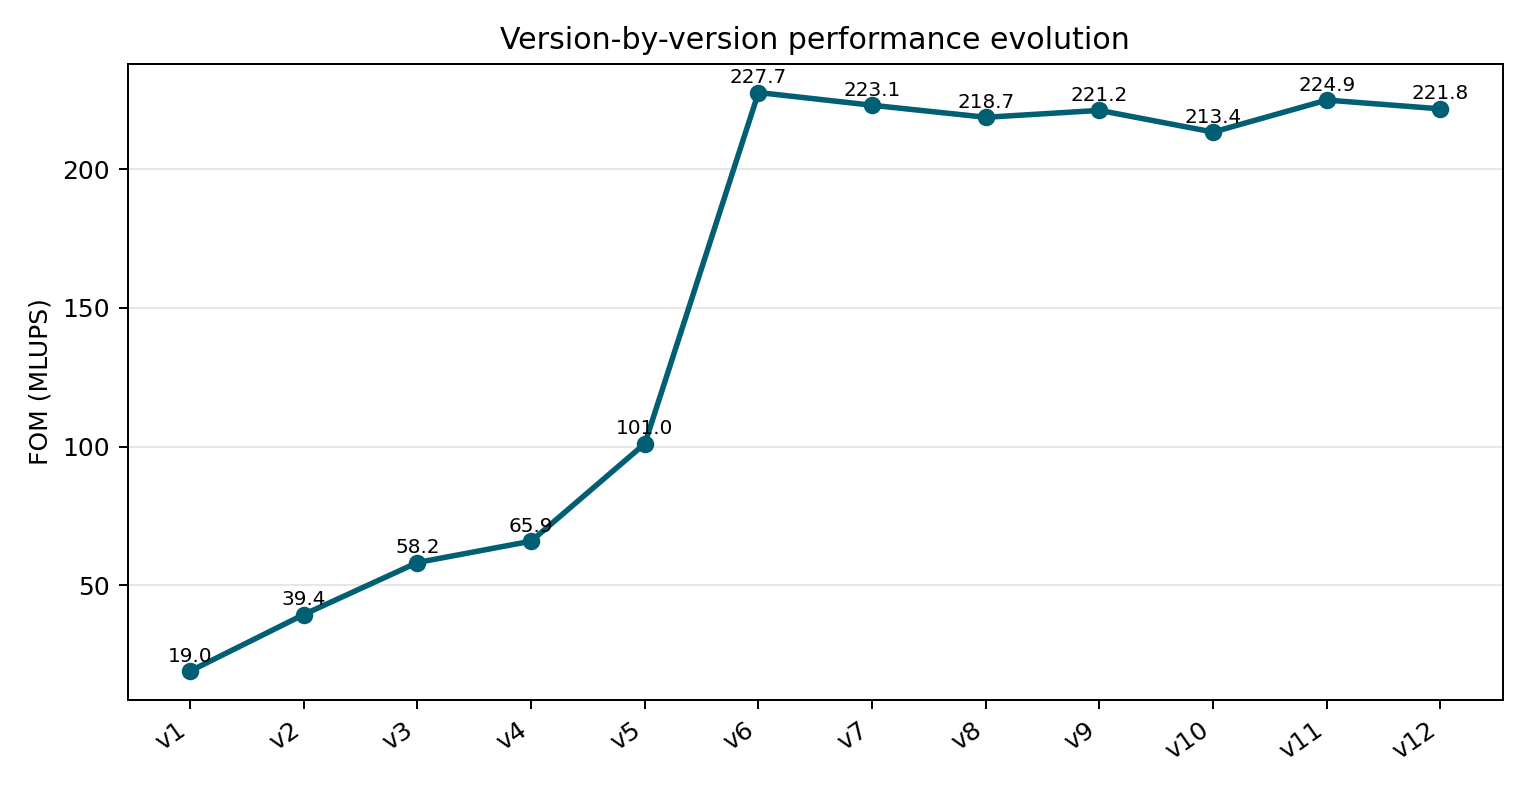
\includegraphics[width=0.82\textwidth]{report-assets/version_evolution.png}
  \caption{Version-by-version performance evolution from the initial baseline to \texttt{v12}.}
  \label{fig:version-evolution}
\end{figure}

The largest gains came from data-layout improvements, communication restructuring, and the elimination of unnecessary synchronization overhead. In contrast, some intermediate versions plateaued or regressed, which reflects the non-linear nature of performance engineering.

\subsection{Phase A: Single-Core Data Layout and SIMD Improvements}

The first phase focused on improving single-core efficiency by restructuring data access patterns and encouraging vectorization. The main ideas were:
\begin{itemize}[leftmargin=1.5em]
  \item structure-of-arrays oriented organization;
  \item aligned allocations for mesh arrays and communication buffers;
  \item explicit alignment hints to the compiler;
  \item pointer-based inner-loop scans instead of repeated index recomputation.
\end{itemize}

These transformations improved memory locality and reduced address-generation overhead in the dominant kernels.

\begin{table}[H]
  \centering
  \caption{Impact of single-core layout and SIMD-oriented optimizations.}
  \label{tab:phase-a-results}
  \begin{tabular}{@{}llll@{}}
    \toprule
    Version & Main idea & Time (s) & FOM (MLUPS) \\
    \midrule
    v6 & SoA refactor & 35.84 & 72.73 \\
    v10 & Alignment + pointer walk & 24.60 & 105.54 \\
    \bottomrule
  \end{tabular}
\end{table}

\subsection{Phase B: OpenMP Attempts and Negative Scaling}

We then attempted to parallelize the dominant kernels with OpenMP. First, only \texttt{collision()} was threaded; later, OpenMP was extended to both \texttt{collision()} and \texttt{propagation()}. These changes did not improve performance and instead caused measurable regressions.

The main reasons were:
\begin{itemize}[leftmargin=1.5em]
  \item memory-bandwidth contention;
  \item repeated OpenMP runtime overhead;
  \item synchronization costs over many timesteps;
  \item insufficient per-thread workload at the chosen problem size.
\end{itemize}

Table~\ref{tab:openmp-negative} and Figure~\ref{fig:openmp-negative-scaling} illustrate this effect.

\begin{table}[H]
  \centering
  \caption{Example of negative OpenMP scaling.}
  \label{tab:openmp-negative}
  \begin{tabular}{@{}llll@{}}
    \toprule
    Version & Configuration & Time (s) & FOM (MLUPS) \\
    \midrule
    v9 & np=1, omp=1 & 12.51 & 221.64 \\
    v9 & np=1, omp=8 & 15.39 & 176.72 \\
    v9 & np=1, omp=16 & 19.32 & 138.80 \\
    \bottomrule
  \end{tabular}
\end{table}

\begin{figure}[H]
  \centering
  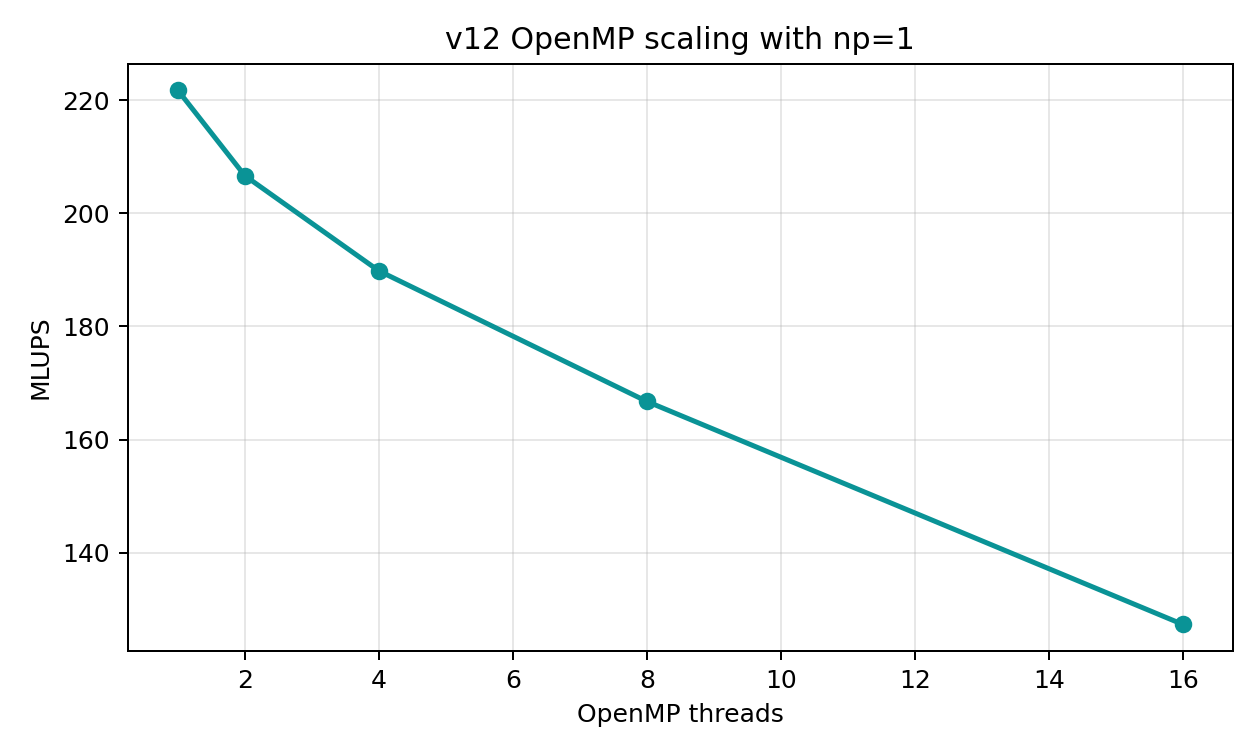
\includegraphics[width=0.75\textwidth]{report-assets/v12_openmp_scaling.png}
  \caption{Representative degradation when increasing OpenMP threads in a single-rank run.}
  \label{fig:openmp-negative-scaling}
\end{figure}

\subsection{Phase C: MPI Halo-Exchange Redesign}

The first major performance breakthrough came from the MPI communication layer. The original halo exchange relied on fragmented blocking communications and excessive synchronization, which made the multi-rank path fragile and inefficient.

The communication scheme was redesigned by:
\begin{itemize}[leftmargin=1.5em]
  \item packing rows, columns, and corner cells into contiguous buffers;
  \item replacing fragmented point-to-point exchanges with \texttt{MPI\_Sendrecv};
  \item removing unnecessary barriers and hidden synchronization overhead.
\end{itemize}

This transformation restored a reliable multi-rank execution path and yielded the first large parallel speedup.

\begin{table}[H]
  \centering
  \caption{Impact of the MPI halo-exchange redesign.}
  \label{tab:mpi-redesign-results}
  \begin{tabular}{@{}llll@{}}
    \toprule
    Version & Configuration & Time (s) & FOM (MLUPS) \\
    \midrule
    Before redesign & np=2, omp=1 & n/a & n/a \\
    After redesign & np=2, omp=1 & 20.27 & 256.85 \\
    \bottomrule
  \end{tabular}
\end{table}

\subsection{Phase D: Single-Thread Fast Path}

After communication had been improved, profiling showed that the best-performing configurations often used \texttt{omp=1}. However, the code still entered OpenMP regions even in effectively serial runs. Dedicated fast paths were therefore introduced to bypass OpenMP runtime overhead when only one thread was used.

This change improved instruction throughput and reduced framework overhead in the main kernels.

\begin{table}[H]
  \centering
  \caption{Impact of serial fast-path specialization.}
  \label{tab:fast-path-results}
  \begin{tabular}{@{}llll@{}}
    \toprule
    Version & Configuration & Time (s) & FOM (MLUPS) \\
    \midrule
    Before fast path & np=2, omp=1 & n/a & 256.85 \\
    After collision fast path & np=2, omp=1 & n/a & 269.57 \\
    After full fast path & np=2, omp=1 & n/a & 276.30 \\
    \bottomrule
  \end{tabular}
\end{table}

\subsection{Phase E: Timestep-Level Synchronization Cleanup}

The final structural optimization removed several explicit \texttt{MPI\_Barrier} calls from the main timestep loop. Since the communication phase already relied on blocking \texttt{MPI\_Sendrecv}, these additional global barriers were redundant and caused unnecessary waiting.

\begin{table}[H]
  \centering
  \caption{Impact of removing redundant timestep barriers.}
  \label{tab:barrier-cleanup-results}
  \begin{tabular}{@{}llll@{}}
    \toprule
    Version & Configuration & Time (s) & FOM (MLUPS) \\
    \midrule
    Before cleanup & np=2, omp=1 & n/a & 276.30 \\
    After cleanup & np=2, omp=1 & n/a & 286.48 \\
    \bottomrule
  \end{tabular}
\end{table}

\section{Scalability Results}

\subsection{Strong Scaling}

The benchmark matrix collected for \texttt{v12} corresponds to a strong-scaling study, since all runs use the same global domain while varying the MPI/OpenMP configuration. This is the most relevant measure for the provided project case, because it directly shows how much faster the reference simulation can be completed when more parallel resources are allocated.

\subsection{MPI/OpenMP Performance Matrix}

An extended benchmark matrix was collected on the local machine for several versions and combinations of MPI ranks and OpenMP threads. Table~\ref{tab:perf-matrix-v12} shows the results for version \texttt{v12}.

\begin{table}[H]
  \centering
  \caption{Performance matrix for version \texttt{v12}.}
  \label{tab:perf-matrix-v12}
  \begin{tabular}{@{}lrrrrr@{}}
\toprule
MPI ranks & OMP=1 & OMP=2 & OMP=4 & OMP=8 & OMP=16 \\
\midrule
1 & 221.78 & 206.67 & 189.84 & 166.74 & 127.29 \\
2 & 375.25 & 356.16 & 290.93 & 233.14 & -- \\
4 & 490.73 & 608.32 & 516.94 & -- & -- \\
8 & 659.93 & 340.57 & -- & -- & -- \\
16 & 657.60 & -- & -- & -- & -- \\
\bottomrule
\end{tabular}

\end{table}

\subsection{Scaling Plots}

Figure~\ref{fig:heatmap-v12}, Figure~\ref{fig:mpi-scaling}, and Figure~\ref{fig:openmp-scaling} illustrate the final scalability trends. Together, they show that MPI-dominant configurations outperform OpenMP-heavy ones on this workload.

\begin{figure}[H]
  \centering
  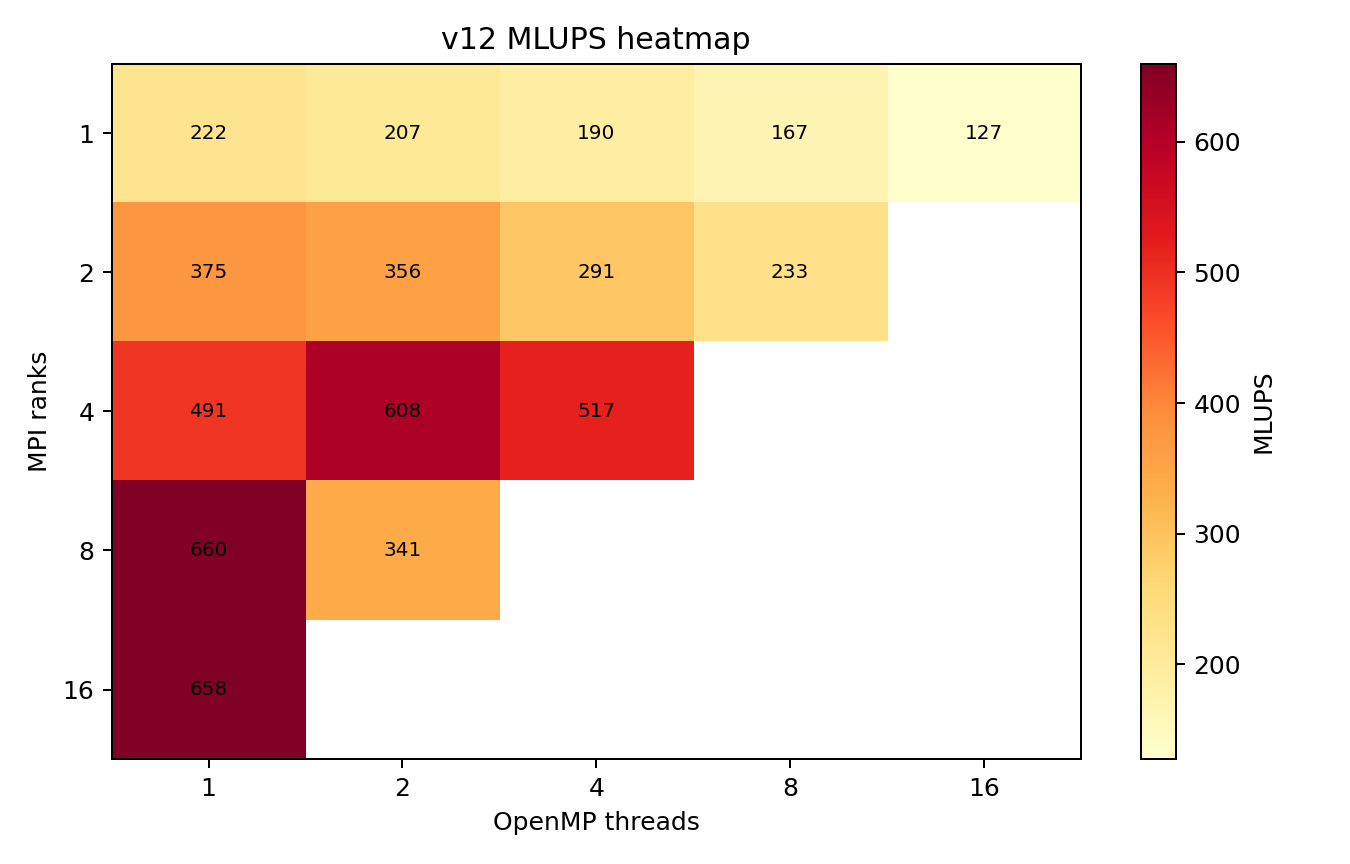
\includegraphics[width=0.75\textwidth]{report-assets/v12_heatmap.png}
  \caption{Heatmap of MLUPS for version \texttt{v12} across MPI/OpenMP configurations.}
  \label{fig:heatmap-v12}
\end{figure}

\begin{figure}[H]
  \centering
  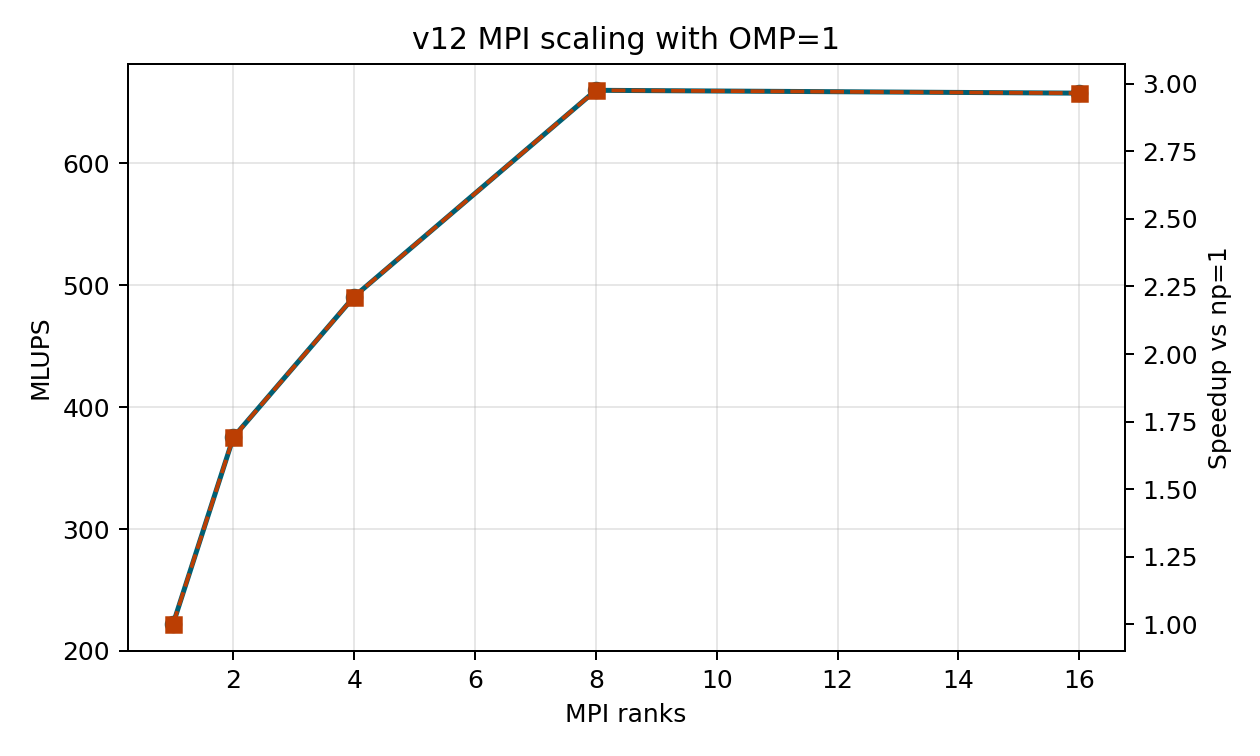
\includegraphics[width=0.75\textwidth]{report-assets/v12_mpi_scaling.png}
  \caption{MLUPS and speedup as a function of the number of MPI ranks for \texttt{OMP=1}.}
  \label{fig:mpi-scaling}
\end{figure}

\begin{figure}[H]
  \centering
  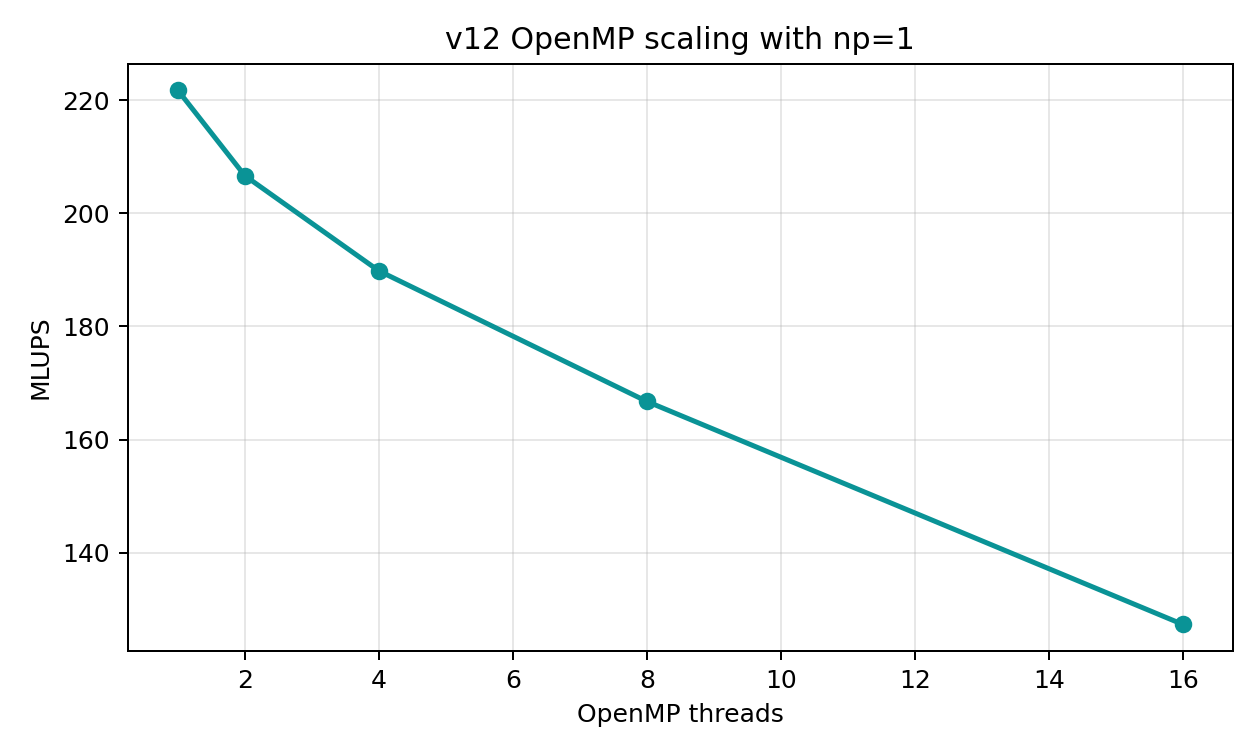
\includegraphics[width=0.75\textwidth]{report-assets/v12_openmp_scaling.png}
  \caption{MLUPS as a function of the number of OpenMP threads for \texttt{np=1}.}
  \label{fig:openmp-scaling}
\end{figure}

The strong-scaling results show a clear asymmetry between distributed-memory and shared-memory parallelism. Increasing the number of MPI ranks significantly improves performance up to the best measured region, while increasing the number of OpenMP threads at fixed \texttt{np=1} consistently degrades performance. This confirms that, for the tested global problem size, communication cleanup enabled profitable MPI scaling, whereas OpenMP runtime overhead and memory-bandwidth contention limited thread-level speedup.

\subsection{Weak Scaling}

Weak scaling evaluates whether the solver can maintain roughly constant performance efficiency when the problem size grows proportionally with the number of processing elements. In this project, a weak-scaling campaign would require generating additional benchmark cases in which the local subdomain size remains approximately constant while the global mesh dimensions increase with the number of MPI ranks.

At the time of writing, the dataset included in this report is centered on the fixed-size reference case and therefore primarily supports strong-scaling conclusions. If additional weak-scaling experiments are performed, they should be reported here using:
\begin{itemize}[leftmargin=1.5em]
  \item a table listing the global domain size, MPI ranks, OpenMP threads, elapsed time, MLUPS, and parallel efficiency;
  \item a plot of weak-scaling efficiency versus the number of MPI ranks;
  \item a short discussion of whether communication costs grow slowly enough to preserve efficiency as the domain expands.
\end{itemize}

If such experiments are added later, this subsection can be replaced by the corresponding figures and tables. Otherwise, the report should explicitly state that only strong scaling was evaluated in depth on the reference benchmark.

\section{Microarchitectural Analysis}

\subsection{Hardware Counter Evidence}

Hardware counters collected with \texttt{perf stat} help explain the observed behavior. For example:
\begin{itemize}[leftmargin=1.5em]
  \item \texttt{v12 np=2 omp=1} reached an IPC of 1.81;
  \item \texttt{v9 np=1 omp=8} only reached an IPC of 0.97.
\end{itemize}

This indicates that the OpenMP-heavy configuration suffered more from stalls, contention, and runtime overhead.

\begin{table}[H]
  \centering
  \caption{Example hardware-counter comparison.}
  \label{tab:perf-stat-comparison}
  \begin{tabular}{@{}lrrrrr@{}}
\toprule
Run & MLUPS & IPC & L1 miss (\%) & Cache miss (\%) & CPUs utilized \\
\midrule
v9-np1-omp8 & 176.72 & 0.97 & 24.77 & 3.88 & 1.68 \\
v12-np2-omp1 & 375.25 & 1.81 & 22.05 & 4.89 & 1.83 \\
\bottomrule
\end{tabular}

\end{table}

\subsection{Hotspot Evolution}

Table~\ref{tab:optimized-hotspots} and Table~\ref{tab:openmp-hotspots} show that after the communication fixes, runtime is once again mostly concentrated in \texttt{collision()} and \texttt{propagation()}, while the OpenMP-heavy path exhibits more thread-runtime overhead.

\begin{table}[H]
  \centering
  \caption{Hotspot distribution for the optimized MPI-oriented configuration \texttt{v12-np2-omp1}.}
  \label{tab:optimized-hotspots}
  \begin{tabular}{@{}lr@{}}
\toprule
Symbol & Samples (\%) \\
\midrule
main & 73.34 \\
collision(Mesh*, Mesh const*) & 37.40 \\
propagation(Mesh*, Mesh const*) & 26.15 \\
lbm\_comm\_halo\_exchange(lbm\_comm\_t\_s*, Mesh*) & 6.38 \\
PMPI\_Sendrecv & 5.09 \\
mca\_pml\_ob1\_send & 4.63 \\
opal\_progress & 2.51 \\
\_\_memmove\_avx512\_unaligned\_erms & 2.66 \\
\bottomrule
\end{tabular}

\end{table}

\begin{table}[H]
  \centering
  \caption{Hotspot distribution for the OpenMP-heavy configuration \texttt{v9-np1-omp8}.}
  \label{tab:openmp-hotspots}
  \begin{tabular}{@{}lr@{}}
\toprule
Symbol & Samples (\%) \\
\midrule
start\_thread & 72.17 \\
collision(Mesh*, Mesh const*) [clone .\_omp\_fn.0] & 31.84 \\
propagation(Mesh*, Mesh const*) [clone .\_omp\_fn.0] & 28.21 \\
clone3 & 31.69 \\
propagation(Mesh*, Mesh const*) & 3.00 \\
GOMP\_parallel & 10.52 \\
main & 7.60 \\
\_\_memmove\_avx512\_unaligned\_erms & 1.62 \\
\bottomrule
\end{tabular}

\end{table}

\section{Negative Results and Dead Ends}

Negative results played an important role in guiding the project. Table~\ref{tab:negative-results} summarizes the main unsuccessful attempts.

\begin{table}[H]
  \centering
  \caption{Summary of negative optimizations and dead ends.}
  \label{tab:negative-results}
  \begin{tabularx}{\textwidth}{@{}lXlX@{}}
    \toprule
    Attempt & Hypothesis & Result & Main reason for failure \\
    \midrule
    OpenMP on \texttt{collision()} & More threads should improve throughput & Regression & Runtime overhead larger than available parallel gain \\
    OpenMP on \texttt{collision()+propagation()} & Larger threaded fraction should scale better & Stronger regression & Memory-bandwidth contention and synchronization \\
    Non-blocking MPI overlap & Communication could be hidden behind computation & No gain & Overlap too small, structural overhead too high \\
    Aggressive arithmetic rewrite & Shorter dependency chain may help vectorization & No gain / instability & Existing kernel already highly optimized; unsafe simplifications \\
    \bottomrule
  \end{tabularx}
\end{table}

\section{Discussion}

A key lesson from this work is that the largest gains did not come from blindly increasing parallelism, but from identifying the right performance model for the application. On this workload, the dominant limiting factors were memory traffic, synchronization, and communication structure rather than raw arithmetic throughput alone.

Another important result is that hybrid parallelism is not automatically superior to MPI-dominant execution. For the tested domain size and machine, MPI scaling was consistently stronger than OpenMP scaling, and many mixed configurations underperformed simpler ones.

\section{Conclusion}

This project transformed a deliberately de-optimized LBM solver into a significantly faster and more scalable implementation. Early gains came from improving data layout, alignment, and vectorization opportunities, but the decisive breakthroughs came from communication redesign and synchronization cleanup.

The final results show that the best configurations were MPI-oriented, with limited or no OpenMP threading. This outcome reflects the memory-bound nature of the solver and the cost of synchronization on the chosen workload. More broadly, the project illustrates that successful optimization requires both low-level kernel tuning and careful restructuring of the global execution flow.

\appendix

\section{Additional Benchmark Data}

Add here any large tables, additional scaling plots, raw \texttt{perf stat} outputs, or extra validation figures that would otherwise overload the main text.

\section{Build and Run Commands}

\begin{lstlisting}[basicstyle=\ttfamily\small,frame=single]
cmake -B build-release -DCMAKE_BUILD_TYPE=Release
cmake --build build-release -j

OMP_NUM_THREADS=1 mpirun -np 2 ./build-release/top.lbm-exe config.txt
\end{lstlisting}

\section{Validation Commands}

\begin{lstlisting}[basicstyle=\ttfamily\small,frame=single]
lbm-viz --check ref_results.raw results.raw
lbm-viz --generate-gif results.raw output.gif
\end{lstlisting}

\end{document}
